%%% This LaTeX source document can be used as the basis for your technical
%%% report. Intentionally stripped and simplified
%%% and commands should be adjusted for your particular paper - title, 
%%% author, citations, equations, etc.
% % Citations/references are in report.bib 

\documentclass[conference]{acmsiggraph}

\usepackage{graphicx}
\graphicspath{{./images/}}
\newcommand{\figuremacroW}[4]{
	\begin{figure}[h] %[htbp]
		\centering
		\includegraphics[width=#4\columnwidth]{#1}
		\caption[#2]{\textbf{#2} - #3}
		\label{fig:#1}
	\end{figure}
}

\newcommand{\figuremacroF}[4]{
	\begin{figure*}[h] % [htbp]
		\centering
		\includegraphics[width=#4\textwidth]{#1}
		\caption[#2]{\textbf{#2} - #3}
		\label{fig:#1}
	\end{figure*}
}


\usepackage{lipsum}

\usepackage{xcolor}
\definecolor{lbcolor}{rgb}{0.98,0.98,0.98}
\usepackage{listings}

\lstset{
	escapeinside={/*@}{@*/},
	language=C,
	basicstyle=\fontsize{8.5}{12}\selectfont,
	numbers=left,
	numbersep=2pt,    
	xleftmargin=2pt,
	%numberstyle=\tiny,
	frame=tb,
	%frame=single,
	columns=fullflexible,
	showstringspaces=false,
	tabsize=4,
	keepspaces=true,
	showtabs=false,
	showspaces=false,
	%showstringspaces=true
	backgroundcolor=\color{lbcolor},
	morekeywords={inline,public,class,private,protected,struct},
	captionpos=t,
	lineskip=-0.4em,
	aboveskip=10pt,
	%belowskip=50pt,
	extendedchars=true,
	breaklines=true,
	prebreak = \raisebox{0ex}[0ex][0ex]{\ensuremath{\hookleftarrow}},
	keywordstyle=\color[rgb]{0,0,1},
	commentstyle=\color[rgb]{0.133,0.545,0.133},
	stringstyle=\color[rgb]{0.627,0.126,0.941},
}


\TOGonlineid{45678}
\TOGvolume{0}
\TOGnumber{0}
\TOGarticleDOI{1111111.2222222}
\TOGprojectURL{}
\TOGvideoURL{}
\TOGdataURL{}
\TOGcodeURL{}

\title{Development of an Android Guitar Tuner Application}

\author{Zoe Wall \\\ 40182161@live.napier.ac.uk \\
Edinburgh Napier University \\
Mobile Applications Development (SET08114)}
\pdfauthor{Zoe Wall}

\keywords{Android, fragments, accelerometer, file I/O, OpenGL}

\begin{document}

\teaser{
   \centering
   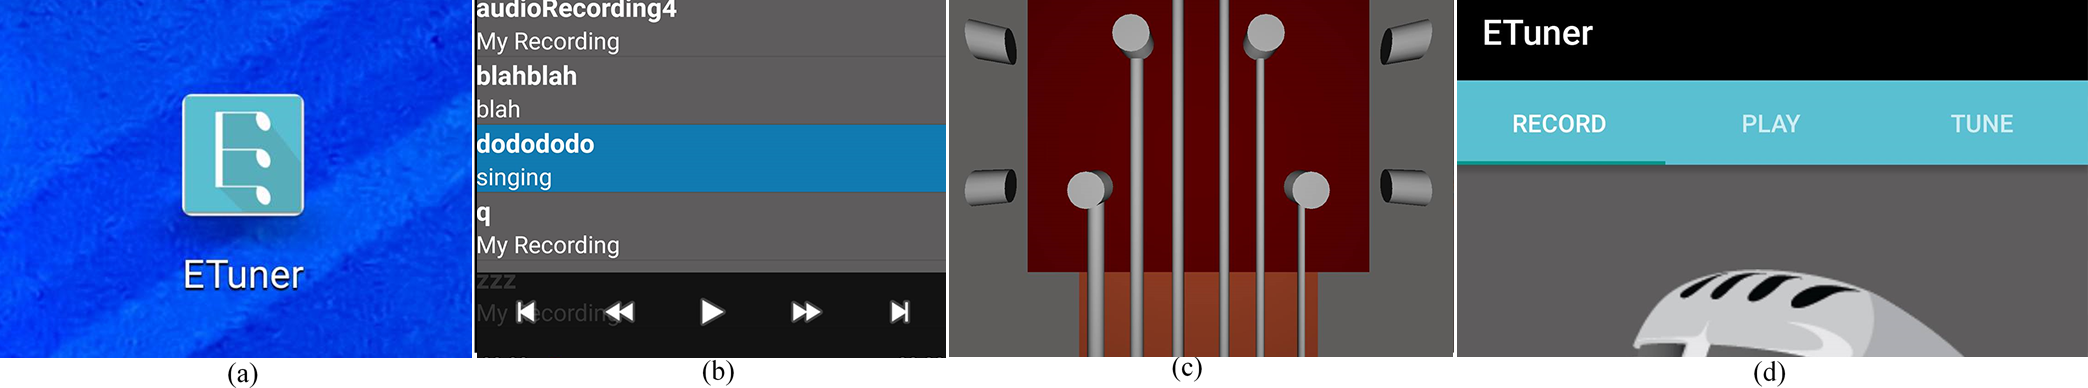
\includegraphics[width=1.0\textwidth]{images/teaser}
   \caption{Project screenshots.}
   \label{fig:teaser}
 }	

\maketitle

\begin{abstract} %% maybe change
This project aims to implement a mobile application prototype using the Android API. The application was intended to be a fully functional guitar tuner and audio recorder, also making use of the OpenGL API for embedded systems, to display 3D graphics. This report details the techniques used, and design decisions made within the development of the application.
\end{abstract}

\keywordlist
%\copyrightspace

%% how to do some stuff
%%\paragraph{Project Aims}

%%\figuremacroW
%%{imagename here}
%%{caption  }
%%{\protect\cite{citteee}}
%%{1.0}

%%\begin{lstlisting}[ caption={display code}]
 	%% CODE HERE
%%\end{lstlisting}

\section{Introduction}

%%An introduction to your assignment stating its scope and content – this
%%should include a brief overview of your application choice and the
%%inspiration for your choice. Reference your reading. 



\section{Software Design}

%%You are expected to do some software modelling of your application choice.
 
\section{Implementation}
%%Short description of your application implementation including screenshots.

\section{Evaluation}
%%4. An evaluation of your implementation. Points to consider discussing in this section are:
%%• A comparison against the original concept as detailed in your introduction
%%• Comparison against other applications/games in the genre, particularly the ones that inspired your choice
%%• An evaluation of your app against user feedback or as compared with other apps/ games
%%• Possible improvements to your application
\section{Summary}

%%Summary of any resources used plus a list of references. You must provide a
%%reference for every resource used that you have not created yourself – for
%%example, images and sound. 



\bibliographystyle{acmsiggraph}
\bibliography{report}


\end{document}